%------------------------------------------------------------------------------%
%                                     FDS                                      %
%------------------------------------------------------------------------------%

\section{FDS}

In this section, we will explain what is \gls{fds}, and we will describe some of
the work that has been realized on this tool.

\subsection{The Fire Dynamics Simulator}

% todo

\subsection{3D loops}

One of the bottleneck of the simulation resides in the computation of the
velocity. This part of the program is composed of three 3D loops that iterates
on the tensors of each mesh, and it can be used several times during a tick of
the simulation. Since it is a critical part of the program, the developers of
\gls{fds} have created a test program, outside the whole simulation, that is
used to measure and try various optimizations. This test program has been very
useful in the effort of optimizing the simulation with \gls{hh} since it was
simple compared to the simulator itself. In this section, we will describe the
test program created by the \gls{fds}'s developers. Then we will explain how the
computation of the velocity has been optimized with the usage of block
decomposition. Finally, we will discuss the limits of the method that has been
used.

\subsubsection{The test program}

As we have seen in the introduction of the section, the test program contains
only the part of the simulation responsible for the computation of the velocity.
The program is composed by three 3D loops parallelized with OpenMP. These loops
are independent, so they are in a parallel section and there are no barriers
between the loops (they run in parallel). The listing \ref{lst:3Dloopscode}
shows the loops with the OpenMP's pragma (all the nested loops are not
represented here).

%- begin listing ------------------------------------------------------------{{{
\begin{listing}[ht!]
\begin{minted}[frame=lines,framesep=2mm,baselinestretch=1.2,fontsize=\normalsize,linenos]{Fortran}
! Compute x-direction flux term FVX

!$OMP PARALLEL PRIVATE(...)
!$OMP DO SCHEDULE(STATIC) PRIVATE(WOMY, VOMZ, TXXP, TXXM, DTXXDX, DTXYDY, DTXZDZ)
DO K=1,KBAR
   ! ...
ENDDO
!$OMP END DO NOWAIT

! Compute y-direction flux term FVY
!$OMP DO SCHEDULE(STATIC) PRIVATE(WOMX, UOMZ, TYYP, TYYM, DTXYDX, DTYYDY, DTYZDZ)
DO K=1,KBAR
   ! ...
ENDDO
!$OMP END DO NOWAIT

! Compute z-direction flux term FVZ
!$OMP DO SCHEDULE(STATIC) PRIVATE(UOMY, VOMX, TZZP, TZZM, DTXZDX, DTYZDY, DTZZDZ)
DO K=0,KBAR
   ! ...
ENDDO
!$OMP END DO NOWAIT
!$OMP END PARALLEL
\end{minted}
\caption{3D loops source code}
\label{lst:3Dloopscode}
\end{listing}
%- end listing --------------------------------------------------------------}}}

The test program is composed in two parts. In the first part, all the variables
are initialized. We will not explain the initialization since it is not present
in the simulator. This initialization is just used to have values on which we
can perform computation. The second part of the program is the computation of
the velocity. We measure the computation time on this part. Finally, the program
computes the mean for each direction (\texttt{FVX}, \texttt{FVY} and
\texttt{FVZ}) in order to have simple values that can be easily verified. The
computation time of the mean is not taken into account when we make the measure
on the original test program unlike on the \gls{hh} program. We will explain why
the \gls{hh} program meausre the computation of the mean as well in the section
\ref{sec:3Dloopsmethod}. Finally, like in the \gls{fds}'s code, most of the
variables are global.

\subsubsection{The method}
\label{sec:3Dloopsmethod}

To introduce \gls{hh} in this first part of the simulation, the idea was to keep
the entire computation in Fortran. The objective was to be efficient and avoid
rewriting the code in C++. Furthermore, all the variables have been kept in
Fortran as well. Here, \gls{hh} has been used as an orchestrator, its role is to
allocated and managed threads in which the Fortran subroutines are called when
it is required. All the OpenMP's pragmas are removed since we do not want to
perform fine grain parallelism, we want the threads to be entirely managed by
\gls{hh}.

As we said in the introduction of this section, to optimize computation time, we
have used block decomposition on the 3D arrays of the simulation. In order to do
this, the Fortran code has been reorganized in subroutines that are parametrized
with the boundaries of the blocks. The loops have been modified to iterate over
the blocks instead of the whole matrix. Then the \gls{hh} tasks manage the
boundaries of the blocks.

%todo

\subsubsection{The results}

% [Computation times] {{{
\begin{figure}[h!]
  \begin{center}
    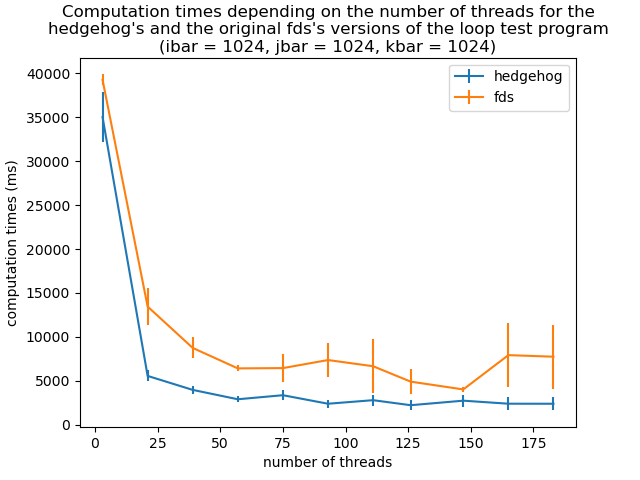
\includegraphics[scale=0.2]{img/fds-loops/times.png}
    \caption{Computation times of the test program for HH and FDS (200 threads node)}
    \label{fig:loopscomptime}
  \end{center}
\end{figure}
%}}}

% [Acceleration] {{{
\begin{figure}[h!]
  \begin{center}
    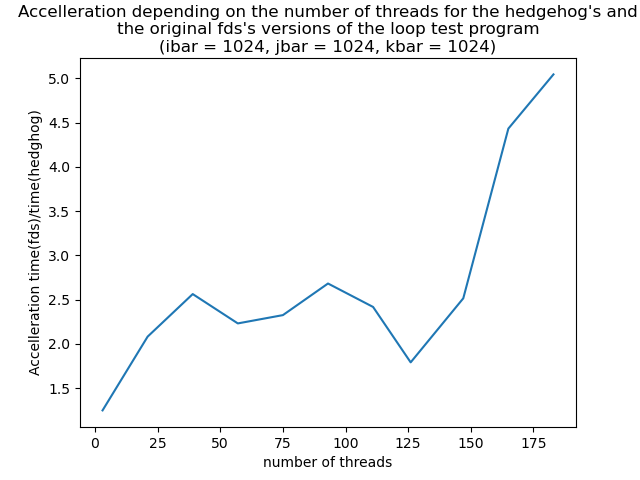
\includegraphics[scale=0.2]{/img/fds-loops/speedup.png}
    \caption{Acceleration of HH over FDS on the test program (200 threads node)}
    \label{fig:label}
  \end{center}
\end{figure}
%}}}

% [Relative speedup] {{{
\begin{figure}[h!]
  \begin{center}
    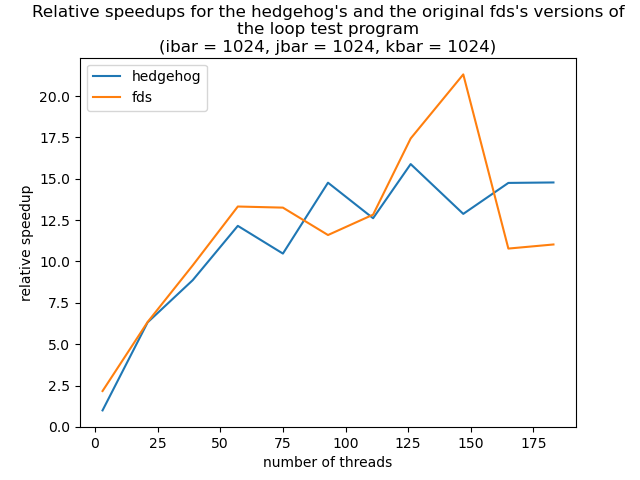
\includegraphics[scale=0.2]{../../img/fds-loops/relative_speedup.png}
    \caption{Relative speedup for HH and FDS on the test program (200 threads node)}
    \label{fig:label}
  \end{center}
\end{figure}
%}}}

\subsubsection{Limits}
